\documentclass[a4paper,12pt]{article}
\usepackage[utf8]{inputenc}
\usepackage{geometry}
\geometry{a4paper, margin=1in}
\usepackage{hyperref}
\usepackage{graphicx}
\usepackage{titlesec}
\usepackage{booktabs}
\usepackage{amsmath}

\titleformat{\section}{\normalfont\Large\bfseries}{\thesection}{1em}{}[\titlerule]

\begin{document}
\begin{center}
    \textbf{\Huge First Lab Report - Group 3}\\
    \vspace{0.2 cm}
    \textbf{\Huge PHY 192}\\
    \rule{\textwidth}{0.4pt}
\end{center}

\vspace{1cm}

\noindent \textbf{\LARGE Question 3.1}

\vspace{0.4cm}

In this first report, our group (Group 3) explores the refractive indices of lenses composed of different materials.

\vspace{0.3cm}

For the first part of the experiment, we aim to determine the index of refraction of a C-shaped lens by studying how it bends light when a red laser beam is shone through it.

\vspace{0.1cm}

Specifically, we will analyze the refraction angle (dependent variable) produced by the lens when the laser is incident at different angles (independent variable).

\vspace{0.1cm}

The relationship between the dependent and independent variables is governed by a fundamental equation in optics: Snell's Law. This equation is given by:

\begin{equation}
    n_1 \sin(\theta_1) = n_2 \sin(\theta_2)
\end{equation}

\vspace{0.1cm}

where $n_1$ and $n_2$ are the refractive indices of the two materials. The refractive index is defined as the ratio of the speed of light in a vacuum to the speed of light in the material. The angles $\theta_1$ and $\theta_2$ represent the angles of incidence and refraction, respectively.

\vspace{1cm}

\noindent \textbf{\LARGE Question 3.1.1}

\vspace{0.4cm}

If the laser beam does not pass through the center of the lens, refraction will still occur, as light always refracts when transitioning between materials with different refractive indices.

\vspace{0.1cm}

However, a significant issue arises: the angles of incidence and refraction become difficult to measure. The proposed lab setup is designed to simplify the measurement of these angles, but deviation from the intended setup may introduce measurement challenges.

\vspace{8cm}

\noindent \textbf{\LARGE Question 3.1.2}

\vspace{0.4cm}

\begin{figure}[htbp]
    \centering
    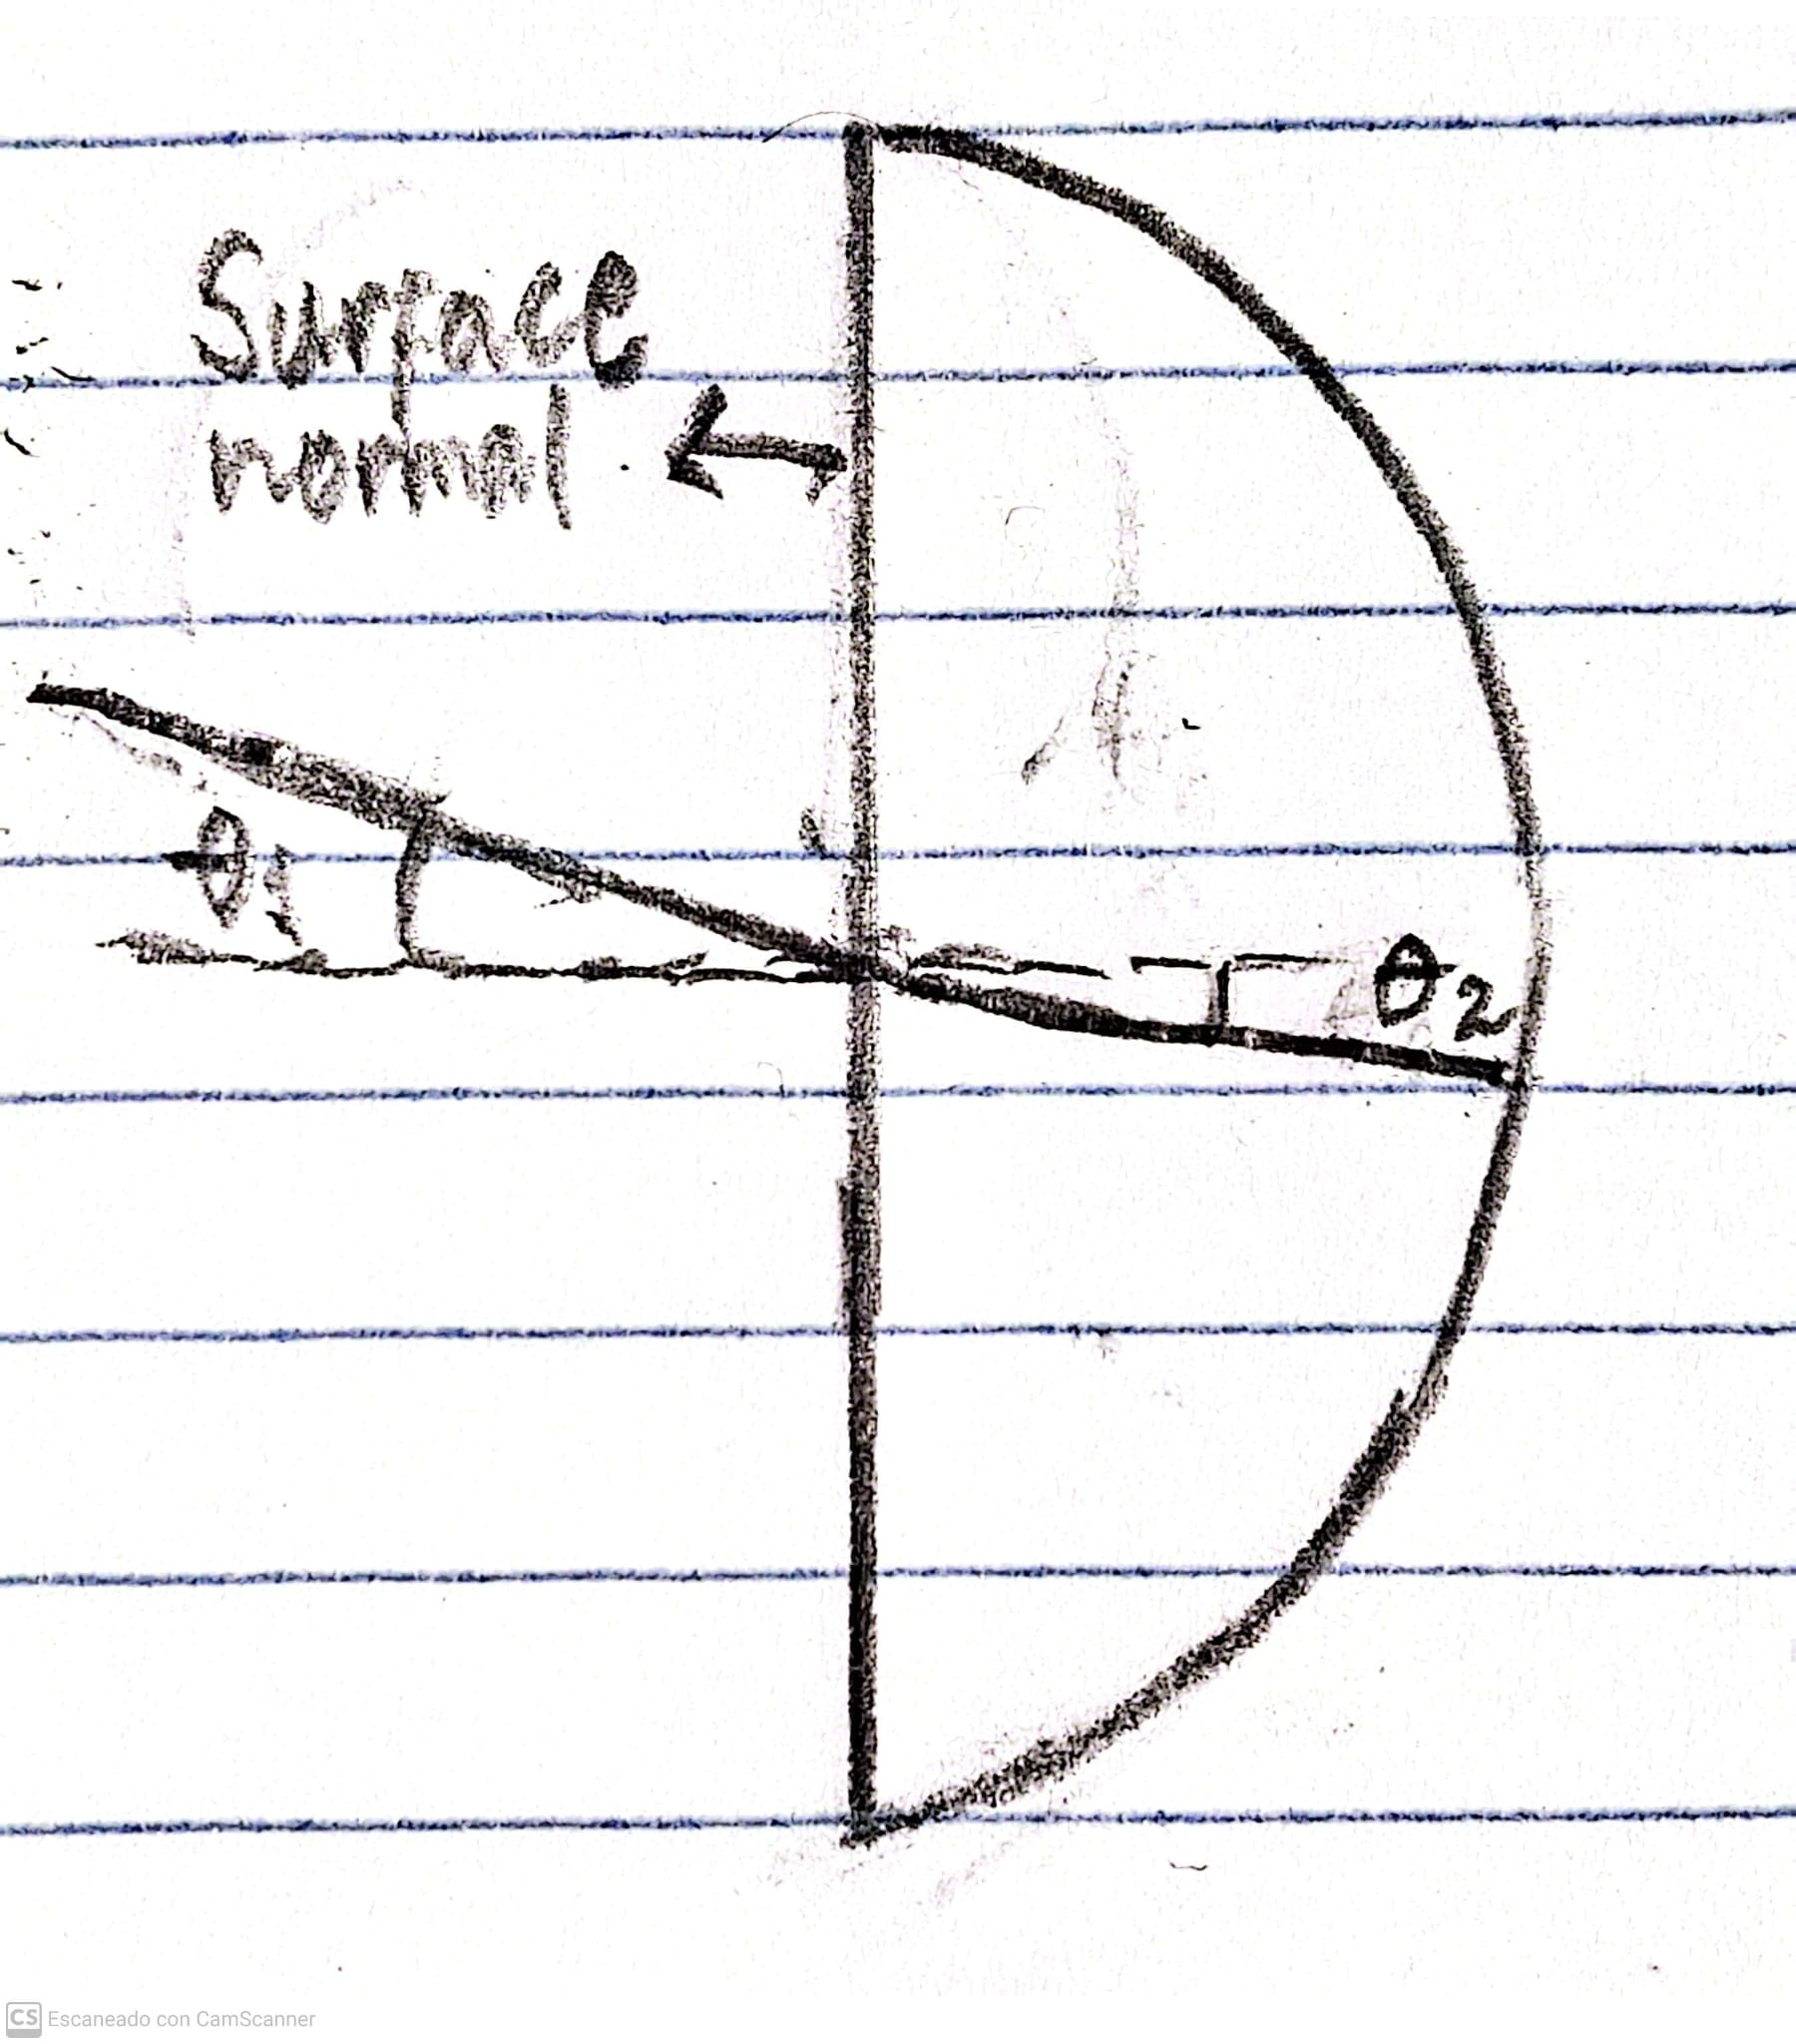
\includegraphics[width=0.5\textwidth]{first_diagram_lab1_PHY_192.jpg}
    \caption{In this diagram the incident angle is marked with the label $\theta_1$ and the refracted angle is marked with the label $\theta_2$, the surface normal is also labeled as such.} 
\end{figure}

\vspace{1cm}

\noindent \textbf{\LARGE Question 3.1.3}

\vspace{0.4cm}

We have that the sine of the angle of incidence is given by: 

\begin{equation}
    \sin(\theta_1) = \frac{n_2}{n_1} \sin(\theta_2)
\end{equation}

We can easily assume that $n_1$ being the refractive index of air is equal to 1, so the equation simplifies to:

\begin{equation}
    \sin(\theta_1) = n_2 \sin(\theta_2)
\end{equation}

It is also physically impossible for the refractive index of the lens to be less than 1 because that would imply that light is going faster than the speed of light in a vacuum which isn't possible. As such we can assume that $n_2 > 1$, as such we know as a fact that the sine of the angle of incidence is always less than or equal to 1, so we can conclude that the refracted angle is always more than the incident angle.

\vspace{0.1cm}

As the sine of an angle is directly proportional to the angle itself, we can conclude that the refracted angle is always greater than the incident angle.

\vspace{3cm}

\noindent \textbf{\LARGE Question 3.1.4 - 3.1.6}

\vspace{0.4cm}

\begin{table}[h]
    \centering
    \begin{tabular}{cccccc}
        \toprule
        $\theta_0$ & $\theta_1$ & $\theta_{2L}$ & $\theta_{2R}$ & $\theta_2$ avg & $d\theta_2$ \\
        \midrule
        0  & 10  & 5  & 7  & 6   & 0.5 \\
        0  & 20  & 10 & 15 & 12.5 & 0.5 \\
        0  & 30  & 15 & 21 & 18   & 0.5 \\
        0  & 40  & 21 & 26 & 23.5 & 0.5 \\
        0  & 50  & 26 & 33 & 29.5 & 0.5 \\
        \bottomrule
    \end{tabular}
    \caption{Here is a table where $\theta_0$ is the normal angle, $\theta_1$ is the angle of incidence, $\theta_2$ is the angle of refraction, $\theta_{2L}$ and $\theta_{2R}$ are the angles of refraction measured on the left and right side of the lens respectively, and $d\theta_2$ is the uncertainty in the angle of refraction. \textbf{All the angles are measured in degrees.}}
\end{table}

\vspace{1cm}

\noindent \textbf{\LARGE Question 3.1.7}

\vspace{0.3cm}

The following mathematic can be used to do perform the calculations:

\begin{align*}
    n_1 \cdot \sin(\Theta_1) &= n_2 \cdot \sin(\Theta_2) \\
    n_1 &= 1 \\
    n_2 &= n \\
    X &= \sin(\Theta_2) \\
    Y &= \sin(\Theta_1) \\
    \Rightarrow X &= n \cdot Y
    \end{align*}

\vspace{1cm}

\noindent \textbf{\LARGE Question 3.1.9}

\begin{table}[h]
    \centering
    \begin{tabular}{cccccc}
        \toprule
        $X$ & $Y$ & $dX$ & $dY$ \\
        \midrule
        0.1045284633 & 0.1736481777 & 0.004339420389 & 0.004297034447 \\
        0.2164396139 & 0.3420201433 & 0.00425989495 & 0.004100182547 \\
        0.3090169944 & 0.5 & 0.004149766895 & 0.003778748675 \\
        0.3987490689 & 0.6427876097 & 0.004001429434 & 0.003342499437 \\
        0.4924235601 & 0.7660444431 & 0.003797643139 & 0.002804690045 \\
        \bottomrule
    \end{tabular}
    \caption{Here is the table with the requested results.}
    \label{tab:my_label}
\end{table}

\vspace{5cm}

\noindent \textbf{\LARGE Question 3.1.10}

\begin{figure}[htbp]
    \centering
    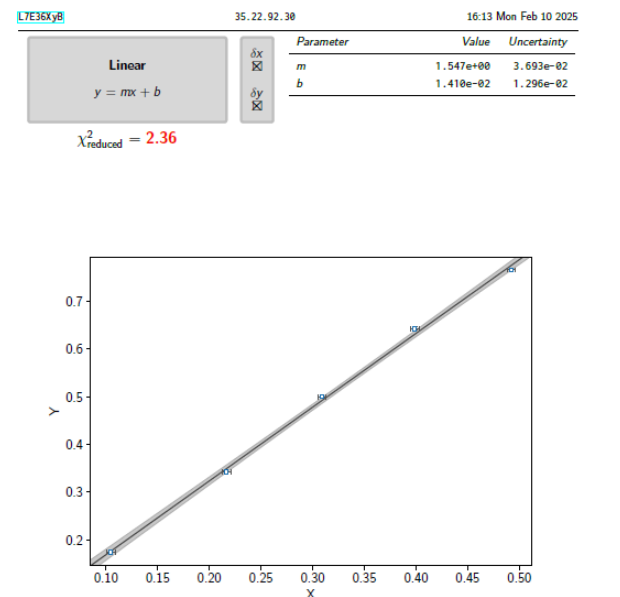
\includegraphics[width=0.5\textwidth]{third_diagram_lab1_PHY_192.png}
    \caption{Here is the plot plus some data relating to the uncertainty of the measurements.} 
\end{figure}

\vspace{1cm}

\noindent Also, for reference the value of $n$ was 1.547, and that of $dn$ was 0.03693

\vspace{15cm}

\noindent \textbf{\LARGE Question 3.2.2}

\begin{figure}[htbp]
    \centering
    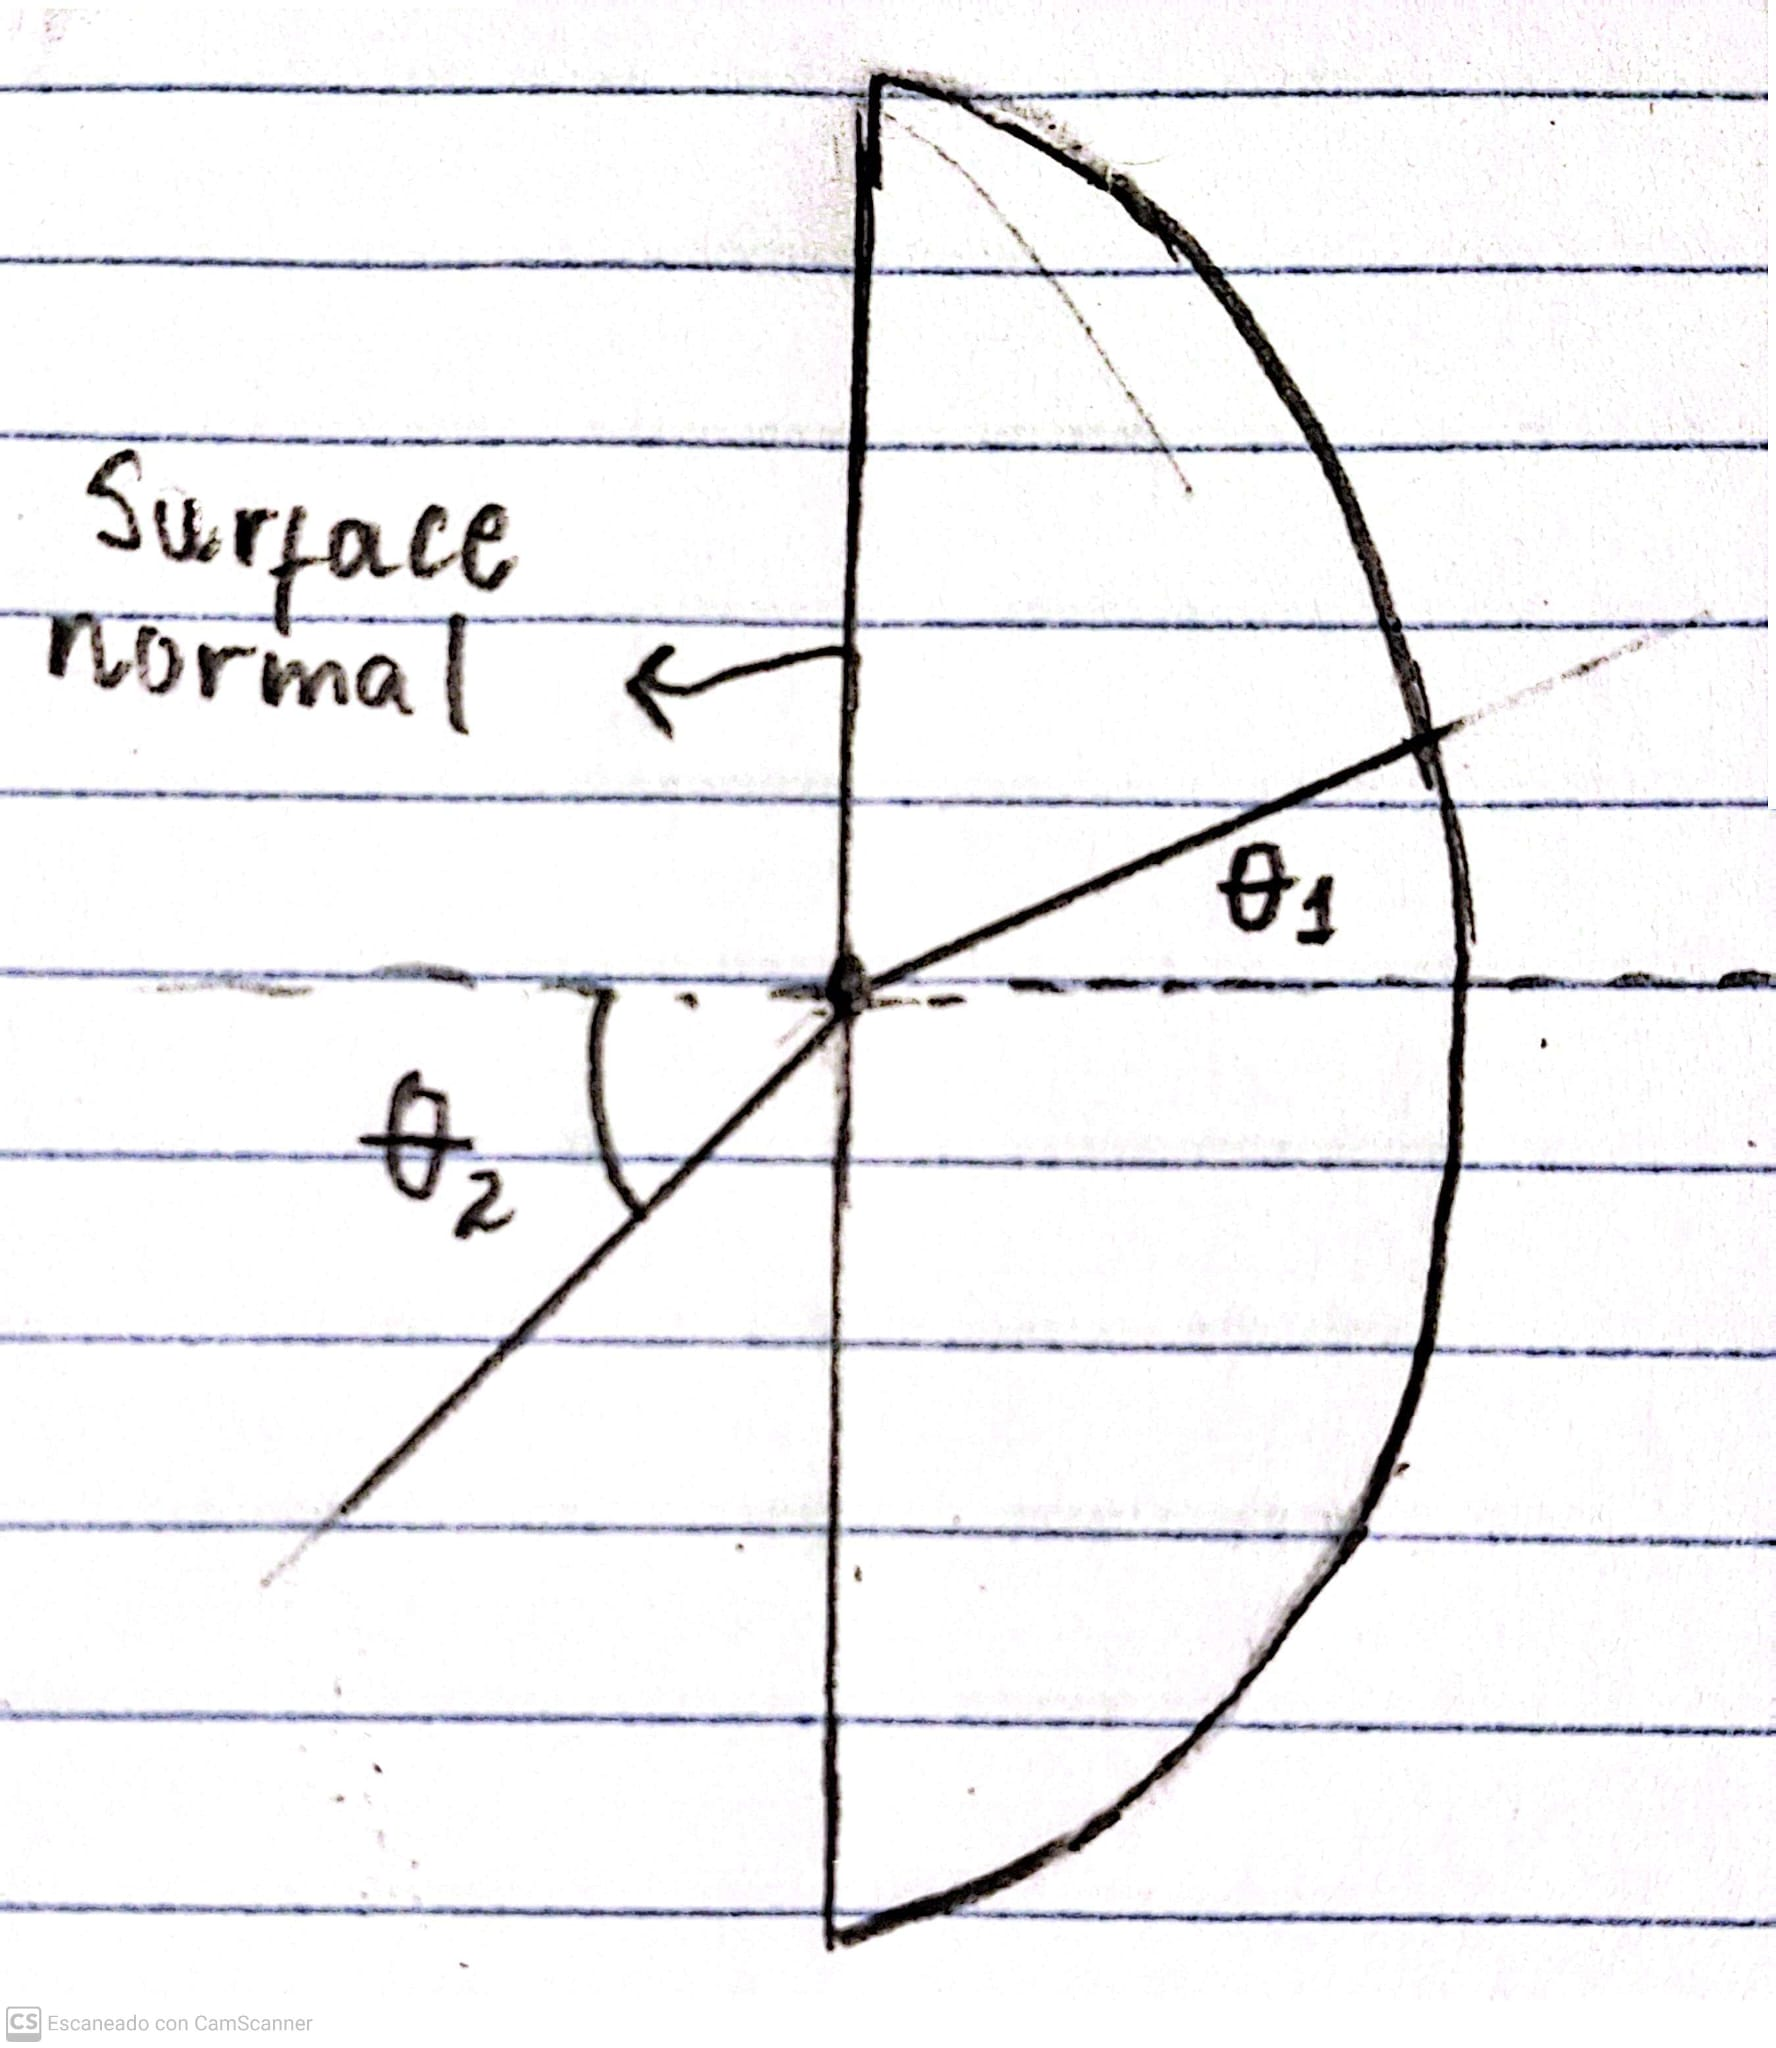
\includegraphics[width=0.5\textwidth]{second_diagram_lab1_PHY_192.jpg}
    \caption{In this diagram the incident angle is marked with the label $\theta_1$ and the refracted angle is marked with the label $\theta_2$, the surface normal is also labeled as such.} 
\end{figure}



\noindent \textbf{\LARGE Question 3.2.3}

\vspace{1cm}

We have that the sine of the angle of incidence is given by: 

\begin{equation}
    \sin(\theta_1) = \frac{n_2}{n_1} \sin(\theta_2)
\end{equation}

We can easily assume that $n_1$ being the refractive index of air is equal to 1, so the equation simplifies to:

\begin{equation}
    \sin(\theta_1) = n_2 \sin(\theta_2)
\end{equation}

It is also physically impossible for the refractive index of the lens to be less than 1 because that would imply that light is going faster than the speed of light in a vacuum which isn't possible. As such we can assume that $n_2 > 1$, as such we know as a fact that the sine of the angle of incidence is always less than or equal to 1, so we can conclude that the refracted angle is always more than the incident angle.

\vspace{0.1cm}

As the sine of an angle is directly proportional to the angle itself, we can conclude that the refracted angle is always greater than the incident angle.

\vspace{0.2cm}

\noindent \textbf{\LARGE Question 3.2.4}

\vspace{0.2cm}

The lens is rotated slowly from one side until the reflected ray no longer emerges after or
before the lens. This is repeated by rotating the lens to the other side. The estimate for the
critical angle is 39 ± 0. 25 degrees. $\frac{1}{sin(39)} = n_1 = 1.59$

\vspace{5cm}

\noindent \textbf{\LARGE Question 3.2.5}

\begin{figure}[htbp]
    \centering
    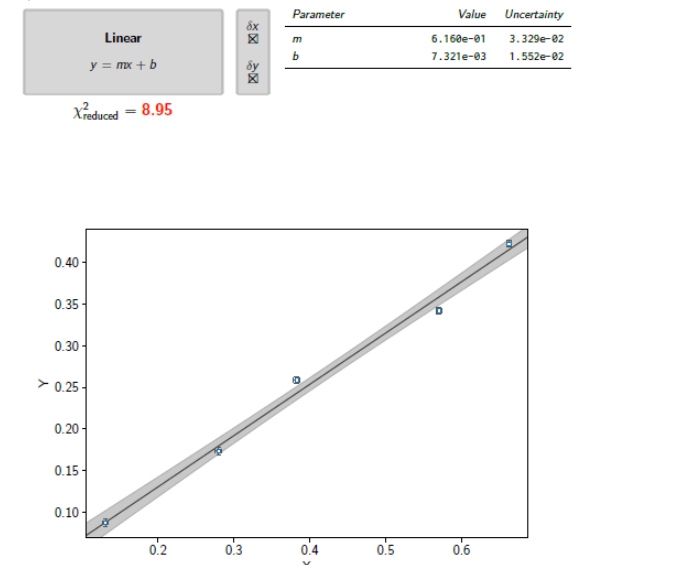
\includegraphics[width=0.5\textwidth]{fourth_diagram_lab1_PHY_192.png}
    \caption{Here is the plot plus some data relating to the uncertainty of the measurements.} 
\end{figure}

\noindent \textbf{\LARGE Question 4.1}

\vspace{0.5cm}

For the first part of the experiment, we aim to determine the deviation angle and the 
deviation of the laser from the normal line associated with a cuboid lens when a red laser beam 
is shone through it. Specifically, we will analyze the refraction angle (dependent variable) 
produced by the lens when the laser is incident at different angles (independent variable). 
The relationship between the dependent and independent variables is governed by the equation:
\[
d = \frac{T}{\cos(\theta_2)} \cdot \sin(\theta_1 - \theta_2)
\]
where $T$ is the thickness of the lens. The angles $\theta_1$ and $\theta_2$ represent the angles of incidence 
and refraction, respectively.

\vspace{1cm}

\noindent \textbf{\LARGE Question 4.2}

\vspace{0.2cm}

\begin{figure}[htbp]
    \centering
    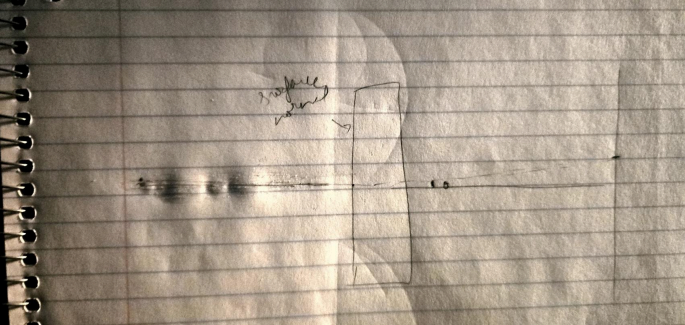
\includegraphics[width=0.5\textwidth]{fifth_diagram_lab1_PHY_192.png}
    \caption{Here is the requested diagram.} 
\end{figure}

\vspace{0.2cm}

\noindent \textbf{\LARGE Question 4.5}

\vspace{0.2cm}

We measured a T value of 25 mm

\vspace{0.2cm}

\noindent \textbf{\LARGE Question 4.7}

\vspace{0.2cm}

\begin{table}[h]
    \centering
    \begin{tabular}{cc}
        \toprule
        Incident Angle ($\theta_1$) & Ideal Deviation (mm) \\
        \midrule
        10 & 0.6616918211 \\
        20 & 2.910497625 \\
        30 & 3.862272453 \\
        40 & 5.012791106 \\
        50 & 4.425952952 \\
        \bottomrule
    \end{tabular}
    \caption{Table showing the ideal deviation of a laser beam for different incident angles when passing through a cuboid lens. The deviation is calculated based on the theoretical model and represents the expected displacement from the normal line.}
    \label{tab:ideal_deviation}
\end{table}

\vspace{0.2cm}

\noindent \textbf{\LARGE Question 4.8}

\vspace{0.2cm}

\begin{table}[h]
    \centering
    \begin{tabular}{cc}
        \toprule
        $\theta_{\text{dev}}$ & $\Delta \theta_{\text{dev}}$ \\
        \midrule
        0.003838308179 & 0.0002473895821 \\
        0.002589502375 & 0.00002094463001 \\
        0.003137727547 & 0.00001820788572 \\
        0.004987208894 & 0.00002480878619 \\
        0.008074047048 & 0.00005891633863 \\
        \bottomrule
    \end{tabular}
    \caption{Table showing the deviation angle ($\theta_{\text{dev}}$) and the uncertainty in the deviation angle ($\Delta \theta_{\text{dev}}$) for different measurements. As requested.}
    \label{tab:deviation_uncertainty}
\end{table}

\end{document}







